\documentclass[12pt,includeheadfoot,a4paper]{report}
\usepackage[print,nopanel]{pdfscreen}
%\begin{print}
\usepackage{lipsum}% http://ctan.org/pkg/lipsum
\usepackage{titletoc}% http://ctan.org/pkg/titletoc
%\section{type}
%\usepackage{sagetex}

\usepackage{listings}
\bibliographystyle{ieeetr}

\usepackage{lastpage}
\usepackage{macro/macro}
\usepackage{float}
\usepackage{fancyhdr}
\usepackage{verbatim}
\usepackage[Glenn]{fncychap}
\lhead{\bfseries OpenSCAD's Customizer}
\rhead{}
\usepackage[left=2.5cm, right=1.5cm, top=1.5cm, bottom=1.5cm]{geometry}
\pagestyle{fancy}
%\end{print}
\margins{2.5cm}{1.5cm}{1.5cm}{1.5cm}
\begin{screen}

\renewcommand{\encodingdefault}{T1}
\usepackage{setspace}
\linespread{1.5}
\renewcommand{\rmdefault}{ptm}
\end{screen}
\screensize{8cm}{9cm}
\overlay{overlay8.pdf}
\usepackage{graphicx}

\begin{document}
\newcommand{\centertext}[1]{\begin{center}\textbf{#1}\end{center}}
\newcommand{\student}{\vskip 2.5cm}
\newcommand{\supervisor}{\vskip 2cm}
\newcommand{\stamp}{\vskip 2.5cm}
\newcommand{\HRule}{\rule{\linewidth}{0.5mm}}
\newcommand{\projecttitle}{\Huge \bf{thepoet.me}}
\newcommand{\tab}[1]{\hspace{.4\textwidth}\rlap{#1}}
\newcommand{\itab}[1]{\hspace{.05\textwidth}\rlap{#1}}
\newcommand{\logo}[1]{\includegraphics[scale=0.16]{#1}}
\newcommand{\submitted}{
\vskip 0.4in
\textnormal{Submitted for partial fulfilment of the Degree\\
of\\
Bachelor of Technology\\
(Information Technology)\\
}
\vskip 2.5cm
%\image{0.7}{images/gne.png}{}

\includegraphics[width=7cm]{images/gne.png}
\vskip 2.5cm
\begin{minipage}{0.4\textwidth}
\begin{flushleft} \large
{Submitted by:}\\
\textnormal{Jagjeet Singh\\
1411266\\146034} % Your name
\end{flushleft}
\end{minipage}
~
\begin{minipage}{0.4\textwidth}
\begin{flushright} \large
{Submitted to:} \\
\textnormal{Sidharath Jain\\Training Coordinator\\IT Department \\                                                                                     } % Supervisor's Name
\end{flushright}
\end{minipage}\\[1.55cm]
\HRule \\[0.4cm]

\textnormal{Information Technology\\
\textbf{Guru Nanak Dev Engineering College} \\
Ludhiana 141006}
}


\newcommand{\pagetitle}{\begin{center}
\projecttitle
\Large\textbf{}\\
\submitted
\vskip 1cm

\end{center}}
\newcommand{\openoffice}{\textbf{OpenOffice}}
\newcommand{\frontmatter}[1]{\begin{Large} \textbf{#1} \end{Large}}
\newcommand{\ppttitle}{\begin{center}
\end{center}}


\begin{screen}
\ppttitle
\end{screen}

\thispagestyle{empty} 
\pagetitle
\newpage
\pagenumbering{Roman}
\cfoot{\thepage}

\begin{Large}
\centertext{Abstract}
\end{Large}

Thepoet.me (Usually styled as thepoet.me)  is a Django based site that I worked upon for my 6-month training. The site offers registered user a simple platform from which to link his/her published book and popular social networking websites such as Facebook, Twitter and Instagram. It is characterized by its one-page user profiles, each with a large, often-artistic background and abbreviated biography. It is a free and Open-source application. The site is fully responsive with all type of devices.

Your thepoet.me acts as a virtual online business card. Put the URL to your site in your e-mail as digital signature, Twitter profile, share it on Facebook, add it to your Instagram as a website.

If you are a poet or writer of some sort who doesn't have a website, you can point colleagues, clients, and prospects to your thepoet.me page so they can find out more about you and connect with you in all the right places.

There are countless platforms out there that you can use to build your own free personal website, but not all of them will deliver the same sense of quality and professionalism. If you’re a poet or writer and looking for something fast and simple that you just need to represent a landing page for yourself, thepoet.me could be one of your best alternatives to choose from.

Other website and blog building tools like Blogger and WordPress.com offer a complete platform to build upon, including the ability to host several web pages, write blog posts and feature widgets. thepoet.me gives you just one, single page to display all your links and a summary of yourself, making it an ideal tool to get straight to the point about you and your published books.

\newpage
\begin{Large}
\centertext{Acknowledgement}
\end{Large}

I, student of Guru Nanak Dev Engineering College, Ludhiana, have taken efforts in this project.
However, it would not have been possible without the kind support and help of many individuals
and organizations. I would like to extend my sincere thanks to all of them.\\

The author is highly grateful to Dr. Sehijpal Singh, Guru Nanak Dev Engineering College, Ludhiana for providing him with the opportunity to carry out his Six Weeks Training at
Testing and Consultancy Cell, Guru Nanak Dev Engineering College, Ludhiana.\\

The author would like to wholeheartedly thank Dr. H.S. Rai Dean, Testing and Consultancy
Cell, Guru Nanak Dev Engineering College, Ludhiana who is a vast sea of knowledge and without whose constant and never ending support and motivation, it would never have been possible to complete the project and other assignments so efficiently and effectively.\\

Finally, I would thank's Nirbhay Chauhan and My Mentors at FreeCAD organization Yorik van Havre, Bernd Hahnebach and whole FreeCAD community. Without their encouragement and Guidence, it would not have been possible to complete this project
in such an efficient manner.

\vskip 1.0cm 
\noindent Amritpal Singh


\newpage
\tableofcontents
\newpage
\listoffigures
\newpage
\listoftables
\newpage


\pagenumbering{arabic}
\cfoot{\thepage}

\newpage
\chapter{INTRODUCTION OF ORGANIZATION}
\begin{figure}[ht]
\centering
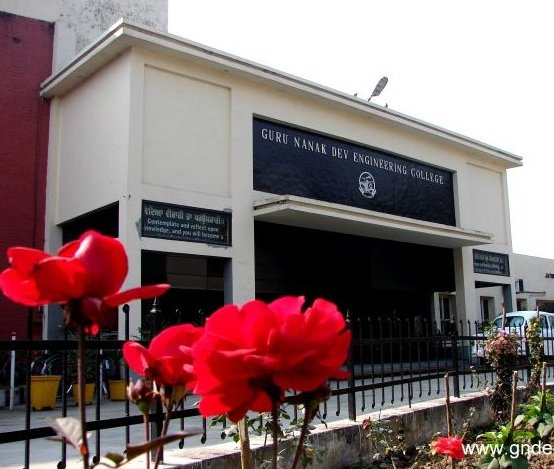
\includegraphics[scale=0.5]{images/gndec.jpg}
\caption{Guru Nanak Dev Engineering College}
\end{figure}
\hspace{-1.7em} I had my Six Month Industrial Training at TCC-Testing And Consultancy Cell, GNDEC Ludhiana. Guru Nanak Dev Engineering College was established by the Nankana
Sahib Education Trust Ludhiana. The Nankana Sahib Education Trust i.e NSET
was founded in memory of the most sacred temple of Sri Nankana Sahib, birth place
of Sri Guru Nanak Dev Ji. With the mission of Removal of Economic Backwardness
through Technology Shiromani Gurudwara Parbandhak Committee i.e SGPC started a
Poly technical was started in 1953 and Guru Nanak Dev Engineering College was established in 1956.\\


The main goal of this institute is:
\begin{itemize}
\item To build and promote teams of experts in the upcoming specialisations.
\item To promote quality research and undertake research projects keeping in view their
relevance to needs and requirements of technology in local industry.
\item To achieve total financial independence.
\item To start online transfer of knowledge in appropriate technology by means of establishing multipurpose resource centres.
\end{itemize}
\section{Testing and Consutancy Cell}

I had my Six Month Institutional Training at TCC i.e Testing And
Consultancy Cell,
GNDEC Ludhiana under the guidance of Dr. H.S.Rai Dean Testing and Consultancy Cell.
Testing and Consultancy Cell was established in the year 1979 with a basic aim to produce
quality service for technical problems at reasonable and affordable rates as a service to society
in general and Engineering fraternity in particular.\\

Consultancy Services are being rendered by various Departments of the College to the
industry, Sate Government Departments and Entrepreneurs and are extended in the form of
expert advice in design, testing of materials \& equipment, technical surveys, technical audit,
calibration of instruments, preparation of technical feasibility reports etc.
This consultancy cell of the college has given a new dimension to the development
programmers of the College. Consultancy projects of over Rs. one crore are completed by the
Consultancy cell during financial year 2009-10. \\

Ours is a pioneer institute providing Consultancy Services in the States of Punjab, Haryana,
Himachal, J\&K and Rajasthan. Various Major Clients of the Consultancy Cell are as under:\\
\begin{itemize}
\item Northern Railway, Govt. of India
\item Indian Oil Corporation Ltd.
\item Larson \& Turbo.
\item Multi National Companies like AFCON \& PAULINGS.
\item Punjab Water Supply \& Sewage Board
\end{itemize}


\newpage


\chapter{Introduction To Project}

\section{Overview}

Thepoet.me(Usually styled as thepoet.me)  is a Django based site that I worked upon for my 6-month training. The site offers registered user a simple platform from which to link his/her published book and popular social networking websites such as Facebook, Twitter and Instagram. It is characterized by its one-page user profiles, each with a large, often-artistic background and abbreviated biography. It is a free and Open-source application. The site is fully responsive with all type of devices.

Your thepoet.me acts as a virtual online business card. Put the URL to your site in your e-mail as digital signature, Twitter profile, share it on Facebook, add it to your Instagram as a website.

If you are a poet or writer of some sort who doesn't have a website, you can point colleagues, clients, and prospects to your thepoet.me page so they can find out more about you and connect with you in all the right places.

There are countless platforms out there that you can use to build your own free personal website, but not all of them will deliver the same sense of quality and professionalism. If you’re a poet or writer and looking for something fast and simple that you just need to represent a landing page for yourself, thepoet.me could be one of your best alternatives to choose from.

Other website and blog building tools like Blogger and WordPress.com offer a complete platform to build upon, including the ability to host several web pages, write blog posts and feature widgets. thepoet.me gives you just one, single page to display all your links and a summary of yourself, making it an ideal tool to get straight to the point about you and your published books.

The main idea of this project is to provide a personal identity page to poets or writers with features to link their published book and social networking sites. User Interface is designed in a way such that layman can easily understand it. The core part of this project is implemented using Django and for GUI part Bootstrap is used. My training being not based on particular language or technology, different types of open-source software’s and technologies are used in this project and many during my training which are not used in this project like Android for Nitnem, Jekyll for blog and shell scripting for plzalert.me

My training being not based on particular language or technology, different type of open-source software's and technologies are
used in this project and many during my training which are not used in this
project like Django, Facebook's Graph API for\emph{plzalert.me} WebApp.

\section{The Existing System}
At present, the rebar functionality in FreeCAD is very limited and creating a reinforcement system is quite tedious. The current approach is followed by creating a sketch for the rebar profile and defining the required set of constraints. This becomes very time-consuming task when user has building model with several structural objects. We can only creates planar rebars by using current rebar tool. 

{\bf {Limitations of previous system }}
\begin{itemize}
	
	\item The AST of Rebar object was not strong.
	
	\item It creates only planar rebars.
	
	\item Circular dependencies issue with Arch structural object.
	
	\item Lack of User interface.
	
	\item No default rebar shapes present.
	
	\item Complex workflow.
	
	\item Rebar object not calculates its rebar length.

    \item Reinforcing rebars in real building model is very time-consuming task.
	
\end{itemize}

\section{User Requirement Analysis}
User Requirements Analysis for a software system is a complete description of the requirements of the User. It includes functional Requirements
and Non-functional Requirements. Non-functional requirements are
requirements which impose constraints on the design or implementation.

 
{\bf Users of the System:}
    \begin{enumerate}
        \item \textbf{Poet or writer:} A poet is a person who writes poetry. A poet may simply be a writer of poetry.
        \item \textbf{Author:} A writer of a book, article, or document.        
    \end{enumerate}

\subsection{Functional Requirements}
\begin{itemize}
    \item  {\bf Specific Requirements}: This phase covers the whole requirements for the system. After
    understanding the system we need the input data to the system then we watch the output
    and determine whether the output from the system is according to our requirements or not.
    So what we have to input and then what well get as output is given in this phase. This phase
    also describe the software and non-function requirements of the system.

    \item {\bf Input Requirements of the System}:
    \begin{itemize}
     \item \textbf{Social Login/Signup:} This means there should be an option so that a user can Login or Register as new user using his/her social accounts. (Facebook, Gmail)
     \item \textbf{Signup:} This means there should be an option so that a user can register.
     \item \textbf{Login:} This means there should be an option so that a user can login after successful registration.
     \item \textbf{Password Reset:} This means there should be an option so that a user can change his/her password.
     \item \textbf{Lost Password:} This means there should be an option so that a user can set a new password in case he/she forgot the old one.
     \item \textbf{Edit Profile:} This means there should be an option so that a user can edit his/her profile anytime after successful login.
     \item \textbf{User profile Link:} This means there should be an option so that a user can copy his profile link.
     \item \textbf{Social networking links:} This means there should be an option so that a user can add his/her Facebook, Twitter and Instagram links. 
     \item \textbf{Book Cover:} This means there should be an option so that a user can add his/her book’s cover and details.

     \end{itemize}

\end{itemize}
\subsection{Non-functional requirements}
\begin{enumerate}
   \item E-mail should be sent using time of registration or password reset.
   \item User web page should be shown after clicking on his/her profile link.
   \item Site should be fully responsive.
\end{enumerate}


\section{Feasibility Study}
Feasibility study aims to uncover the strengths and weaknesses of
a project. In its simplest term, the two criteria to judge feasibility
are cost required and value to be attained. As such, a well-designed
feasibility analysis should provide a historical background of the
project, description of the project or service, details of the
operations and management and legal requirements. Generally, feasibility
analysis precedes technical development and project implementation.
These are some feasibility factors by which we can determine that
the project is feasible or not:
\begin{itemize}
\item {\bf{Technical feasibility}}: Technological feasibility is carried
out to determine whether the project has the capability, in terms of
software, hardware, personnel to handle and fulfill the user requirements. This whole project is based on Open
Source Environment and is part of an open source software which would be deployed on any OS.

\item {\bf{Economic feasibility}}: In Economic feasibility, we
determine whether the benefit is gain according to the cost invested
to develop the project or not. If benefits outweigh costs, only then
the decision is made to design and implement the system. It is
important to identify cost and benefit factors, which can be categorized
as follows:

\begin{enumerate}
\item Development costs.
\item Operating costs.
\end{enumerate}
Thepoet.me is also Economically feasible for a year as It could be developed and maintain with zero cost as It is supported by Open source community and GitHub Students Pack.
\end{itemize}



\section{Objective of Project}

To ease up the rebaring process in FreeCAD, an interactive addon is developed where user will input the required data as per the design requirements and they will need not to draw rebars from the Sketcher workbench for creating reinforcement in the structural object.

One of the primary benefits of this addon is the ability to create parametric rebars. These are designs which are parametrized using parameters or top-level variables.

\begin{enumerate}
    \item Provides full GUI (Graphical User Interface) for reinforcing rebars in the structural object.
    \item They also requires pre-built standard rebar shapes.
    \item Different rebars will have their own view and data properties.
    \item User can edit the parameters of the group of rebars from the view \& data properties itself.
    \item These rebars will be fully parametric. Hence the parameters of the rebars will automatically adjust themselves if the changes are made to their parent structure.
%    \item Easy to use. 
\end{enumerate}


%The major Objectives of this project are:
%\begin{enumerate}
%    \item Syntax support for generation of customization form:
%    The customization form generated on Thingiverse is based on a certain syntax for both describing the elements in the form and providing a range of their values. In order to make this work in OpenSCAD as well, the same style of description and parameterization can be incorporated into OpenSCAD. Hence the user will be able to generate the customization form from within OpenSCAD by adding a few simple lines in the .scad file.
%  
%    Customization of the model from the form:
%    Once the form is ready, it must be able to customize the model as desired by the user. The changes made in the form should directly correspond to changes in the model itself.
%    Enhancing the UI for the customization form:
%    The customization form is there to make the whole customization thing easy. And that implies that the form itself should also be easy to use. And this can be achieved by having a good and simple look to the whole thing.
%  
%\end{enumerate}




\chapter{PROJECT DESIGN}

\section{Product Perspective}

This site is supposed to be part of an open source, under the GNU general Public License. It offers registered user a simple platform from which to link his/her published book and popular social networking websites such as Facebook, Twitter and Instagram. It is characterized by its one-page user profiles, each with a large, often-artistic background and abbreviated biography.

The following are the main features that are included in thepoet.me

\begin{enumerate}
    \item \textbf{Web Compatibility:} The site easily render on various resolutions, screen sizes, and browsers; and with the increasing popularity of mobile devices, it function properly on the plethora of these types of devices.
    \item \textbf{Search Engine Optimisation:} The site generally receive many visitors, and one method to attract visitors is search engine optimisation. The site is optimised with Google search Engine.
    \item \textbf{Simple and Professional Web Design:} There are countless platforms out there that you can use to build your own free personal website, but not all of them will deliver the same sense of quality and professionalism. If you’re a poet or writer and looking for something fast and simple that you just need to represent a landing page for yourself, thepoet.me could be one of your best alternatives to choose from.
    \item \textbf{Clear, User-friendly Navigation:} The site contain a user-friendly navigation scheme that allows visitors to quickly find the information needed. Important links must be easy to find and given logical, simple, and include easy-to-understand labels. Calls to action are placed in conspicuous spots within the navigation’s scheme.
\end{enumerate}  

\section{Product Functions}

Functions performed by Customizer are:
\begin{itemize}
   
     \item \textbf{Social Login/Signup:} This means there should be an option so that a user can Login or Register as new user using his/her social accounts. (Facebook, Gmail)
     \item \textbf{Signup:} This means there should be an option so that a user can register.
     \item \textbf{Login:} This means there should be an option so that a user can login after successful registration.
     \item \textbf{Password Reset:} This means there should be an option so that a user can change his/her password.
     \item \textbf{Lost Password:} This means there should be an option so that a user can set a new password in case he/she forgot the old one.
     \item \textbf{Edit Profile:} This means there should be an option so that a user can edit his/her profile anytime after successful login.
     \item \textbf{User profile Link:} This means there should be an option so that a user can copy his profile link.
     \item \textbf{Social networking links:} This means there should be an option so that a user can add his/her Facebook, Twitter and Instagram links. 
     \item \textbf{Book Cover:} This means there should be an option so that a user can add his/her book’s cover and details.
     
\end{itemize}


\section{User Characteristics}

We have identified three potential classifications of users of our system:

\begin{enumerate}
    \item Poet or writer: The people who write poetry. A poet may simply be a writer of poetry
    \item Author: The people who are writer of a book, article, or document.
    \item Developers: These are people who might want to integrate new features to thepoet.me

\end{enumerate}

\subsection{The General User}

All users can be assumed to have the following characteristics:

\begin{enumerate}
    \item Ability to read and understand English.
    \item Have at least an e-mail or any social account for registration (Facebook, Google). 
    \item Beyond the above, no further facility with computer technology can be assumed.
\end{enumerate}

\subsection{Developers}
The Developers can be assumed to have the following characteristics:
\begin{enumerate}
    \item Basic Knowledge of programming.
    \item Basic Knowledge of python and Django.
    \item Knowledge of web designing (HTML, CSS, javascript and Bootstrap).
    \item Knowledge of git.
\end{enumerate}

\section{Flowchart}
A flowchart is a type of diagram that represents an algorithm, work flow or process, showing the steps as boxes of various kinds, and their order by connecting them with arrows and the flowchart of customizer showing the flow of control and Data in the software.

\subsection{Detailed Description}

The basic implementation of this project is almost done in form of prototype. There is need to modify the structure of the project. We have to divide the task into there parts:

\begin{enumerate}
	\item \textbf{Front end}
	It will deal with how thepoet.me will look to the user.
	
	\item \textbf{Back End}
	On backend, a top layer is HTML pages render on the user screen but in bottom layer Django (Python Web framework) is running. Django attempts to support as many features as possible on all database backends. However, not all database backends are alike, and we’ve had to make design decisions on which features to support and which assumptions we can make safely.  
	
\end{enumerate}


\section{Class Diagrams}
Class Diagrams describe the static structure of the system. Following classes diagram represent the relationship in thepoet.me:
\begin{enumerate}
	\item Figure \ref{fig:collaborative1} shows the class diagram of the Django ModelForm class which is the base class of accounts.models.Profile.

	\item Figure \ref{fig:collaborative} shows the class diagram of the Django ModelForm class which is the base class of accounts.forms.FirstBookForm.
	
	\item Figure \ref{fig:classAnnotation__coll__graph} shows the class diagram of the accounts.forms.ProfileForm.

\end{enumerate}

\begin{figure}
    \centering
    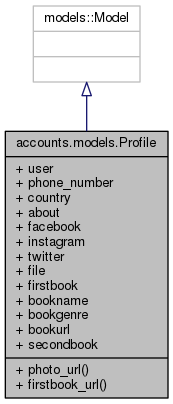
\includegraphics[scale=.85]{images/classaccounts.png}
    \caption{Class Diagram for accounts.models.Profile}
    \label{fig:collaborative1}
\end{figure}

\begin{figure}
    \centering
    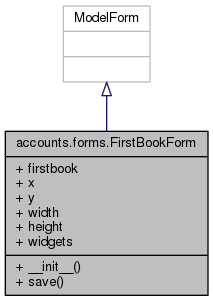
\includegraphics[scale=.85]{images/classacountsform.png}
    \caption{Class Diagram for accounts.forms.FirstBookForm}
    \label{fig:collaborative}
\end{figure}

\begin{figure}
\centering
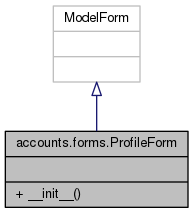
\includegraphics[scale=.85]{images/profileform.png}
\caption{Class Diagram for accounts.forms.ProfileForm}
\label{fig:classAnnotation__coll__graph}
\end{figure}

\section{Dependencies}
Dependencies include softwares or framework that need to be installed for proper working of this software.

This addon could be installed on any given list of operating system.

\begin{enumerate}
	\item Mac OS X
	\item Windows
	 \begin{enumerate} 
	 	\item XP or newer on x86 32/64 bit
	 \end{enumerate}
	\item Linux
	\begin{enumerate} 
		\item Debian 
		\item Ubuntu 
		\item Kubuntu
		\item Arch Linux
		\item openSUSE
		\item Fedora
	 \end{enumerate}
	\item BSD
	\begin{enumerate}
		\item NetBSD  $\geq 6.1$
		\item FreeBSD $\geq 10 $
		\item OpenBSD
	\end{enumerate}
\end{enumerate}	 
 

The main dependencies of rebar addon is FreeCAD (version >=0.17). But If you want to build FreeCAD this software from soucre code on \emph{any OS}, you need some libraries and tools. The version
numbers in brackets specify the versions which have been used for
development. Other versions may or may not work as well.

If you're using a newer version of Ubuntu, you can install these 
libraries from aptitude. If you're using Mac, or an older Linux/BSD, there 
are build scripts that download and compile the libraries from source. 
Follow the instructions for the platform you're compiling on below. Following are
dependencies of FreeCAD software.

\begin{enumerate} 
	\item A C++ compiler supporting C++11
	\item build-essential
	\item python
	\item python-matplotlib
	\item libtool
	\item libcoin60-dev (Debian Wheezy, Wheezy-backports, Ubuntu 13.04 and before)
	\item libsoqt4-dev
	\item libxerces-c-dev
	\item libboost-dev
	\item libboost-filesystem-dev
	\item libboost-regex-dev
	\item libboost-program-options-dev
	\item python-pyside
	\item libqt4-opengl-dev
	\item qt4-dev-tools
	\item libboost-thread-dev
	\item libboost-python-dev
\end{enumerate}



\newpage
\chapter{DEVELOPMENT AND IMPLEMENTATION}
\section{C++}

\begin{figure}[h]
	\centering 
\includegraphics[scale=0.3]{images/c++.png}
	\caption{C++ Logo}
\end{figure}

C++ is a general-purpose programming language. It has imperative, object-oriented and generic programming features, while also providing facilities for low-level memory manipulation.

It was designed with a bias toward system programming and embedded, resource-constrained and large systems, with performance, efficiency and flexibility of use as its design highlights. C++ has also been found useful in many other contexts, with key strengths being software infrastructure and resource-constrained applications, including desktop applications, servers (e.g. e-commerce, web search or SQL servers), and performance-critical applications (e.g. telephone switches or space probes). C++ is a compiled language, with implementations of it available on many platforms and provided by various organizations, including the Free Software Foundation (FSF's GCC), LLVM, Microsoft, Intel and IBM.

C++ is standardized by the International Organization for Standardization (ISO), with the latest standard version ratified and published by ISO in December 2014 as ISO/IEC 14882:2014 (informally known as C++14). The C++ programming language was initially standardized in 1998 as ISO/IEC 14882:1998, which was then amended by the C++03, ISO/IEC 14882:2003, standard. The current C++14 standard supersedes these and C++11, with new features and an enlarged standard library. Before the initial standardization in 1998, C++ was developed by Bjarne Stroustrup at Bell Labs since 1979, as an extension of the C language as he wanted an efficient and flexible language similar to C, which also provided high-level features for program organization.

Many other programming languages have been influenced by C++, including C\#, D, Java, and newer versions of C (after 1998).

Features of Language:
\begin{enumerate}
	\item Object storage
	\begin{enumerate}
		\item Static storage duration objects
		\item Thread storage duration objects
		\item Automatic storage duration objects
		\item Dynamic storage duration objects
	\end{enumerate}
	\item Templates
	\item Objects
	\begin{enumerate}
		\item Encapsulation
		\item Inheritance
	\end{enumerate}
	\item Operators and operator overloading
	\item Polymorphism
	\begin{enumerate}
		\item Static polymorphism
		\item Dynamic polymorphism
		\begin{enumerate}
			\item Inheritance
			\item Virtual member functions
		\end{enumerate}
	\end{enumerate}
\item Lambda expressions
\item Exception handling
\end{enumerate}
\input{input/Development/flex.tex}
\section{Bison}

\begin{figure}[h]
	\centering 
\includegraphics[scale=0.2]{images/gnu.png}
	\caption{GNU Logo}
\end{figure}

Bison is a general-purpose parser generator that converts an annotated context-free grammar into a deterministic LR or generalized LR (GLR) parser employing LALR(1) parser
tables.
Once you are proficient with Bison, you can use it to develop a wide range of language parsers, from those used in simple desk calculators to complex programming languages.


Bison is upward compatible with Yacc: all properly-written Yacc grammars ought to work with Bison with no change. Anyone familiar with Yacc should be able to use Bison with little trouble. You need to be fluent in C or C++ programming in order to use Bison
or to understand this manual. Java is also supported as an experimental feature.


Bison was written originally by Robert Corbett. Richard Stallman made it Yacc-compatible. Wilfred Hansen of Carnegie Mellon University added multi-character string literals and other features. Since then, Bison has grown more robust and evolved many
other new features thanks to the hard work of a long list of volunteers.

Bison .y specification file:

\begin{verbatim}
	/*** Definition section ***/
	
	%%
	
	/*** Rules section ***/
	
	%%
	
	/*** C Code section ***/

\end{verbatim}
\section{Qt}

\begin{figure}[h]
	\centering 
\includegraphics[scale=0.1]{images/qt.png}
	\caption{Qt Logo}
\end{figure}

Qt is a cross-platform application framework that is widely used for developing application software that can be run on various software and hardware platforms with little or no change in the underlying codebase, while still being a native application with native capabilities and speed. Qt is currently being developed both by The Qt Company, a company listed on the Nasdaq Helsinki Stock Exchange and the Qt Project under open-source governance, involving individual developers and firms working to advance Qt. Qt is available with both commercial and open source GPL 2.0, GPL 3.0, and LGPL 3.0 licenses.

Qt is used mainly for developing application software with graphical user interfaces (GUIs); however, programs without a GUI can be developed, such as command-line tools and consoles for servers. An example of a non-GUI program using Qt is the Cutelyst web framework. GUI programs created with Qt can have a native-looking interface, in which case Qt is classified as a widget toolkit.

Qt uses standard C++ with extensions including signals and slots that simplify handling of events, and this helps in development of both GUI and server applications which receive their own set of event information and should process them accordingly. Qt supports many compilers, including the GCC C++ compiler and the Visual Studio suite. Qt also provides Qt Quick, that includes a declarative scripting language called QML that allows using JavaScript to provide the logic. With Qt Quick, rapid application development for mobile devices became possible, although logic can be written with native code as well to achieve the best possible performance. Qt can be used in several other programming languages via language bindings. It runs on the major desktop platforms and some of the mobile platforms. It has extensive internationalization support. Non-GUI features include SQL database access, XML parsing, JSON parsing, thread management and network support.

%\input{input/Development/make.tex}
%\input{input/Development/ctest.tex}
%\input{input/Development/travis.tex}
\section{Introduction to \LaTeX}

\LaTeX, I had never heard about this term before doing this project,
but when I came to know about its features, found it excellent. 
\LaTeX{} (pronounced /ˈleɪtɛk/, /ˈleɪtɛx/, /ˈlɑːtɛx/, or /ˈlɑːtɛk/) is a 
document markup language and document preparation system for the \TeX{} 
typesetting  program. Within the typesetting system, its name is styled 
as \LaTeX.

\image{0.9}{images/donald.png}{Donald Knuth, Inventor Of \TeX{} 
typesetting system}

Within the typesetting system, its name is styled as \LaTeX. The term 
\LaTeX{} refers only to the language in which documents are written, 
not to the editor used to write those documents. In order to create a 
document in \LaTeX, a .tex file must be created using some form of text 
editor. While most text editors can be used to create a \LaTeX{} document, 
a number of editors have been created specifically for working with \LaTeX.

\LaTeX{} is most widely used by mathematicians, scientists, 
engineers, philosophers, linguists, economists and other scholars in 
academia. As a primary or intermediate format, e.g., translating DocBook 
and other XML-based formats to PDF, \LaTeX{} is used because of the 
high quality of typesetting achievable by \TeX. The typesetting system 
offers programmable desktop publishing features and extensive facilities 
for automating most aspects of typesetting and desktop publishing, 
including numbering and cross-referencing, tables and figures, 
page layout and bibliographies.

\LaTeX{} is intended to provide a high-level language that
accesses the power of \TeX. \LaTeX{} essentially comprises a
collection of \TeX{} macros and a program to process \LaTeX documents. 
Because the \TeX{} formatting commands are very low-level, it is usually 
much simpler for end-users to use \LaTeX{}.


\subsection{Typesetting}
\LaTeX{} is based on the idea that authors should be able to focus on 
the content of what they are writing without being distracted by its 
visual presentation. In preparing a \LaTeX{} document, the author 
specifies the logical structure using familiar concepts such as 
chapter, section, table, figure, etc., and lets the \LaTeX{} system 
worry about the presentation of these structures. It therefore 
encourages the separation of layout from content while still allowing 
manual typesetting adjustments where needed. 

\begin{verbatim}
\documentclass[12pt]{article}
\usepackage{amsmath}
\title{\LaTeX}
\date{}
\begin{document}
  \maketitle 
  \LaTeX{} is a document preparation system 
  for the \TeX{} typesetting program.
   \par 
   $E=mc^2$
\end{document}
\end{verbatim}
\image{0.3}{images/latexoutput.png}{\LaTeX{} output of above program.}

\subsection{Installing \LaTeX{} on System}
Installation of \LaTeX{} on personal system is quite easy. As i have used \LaTeX{} on Ubuntu 13.04 so i am discussing the installation steps for Ubuntu 13.04 here:
\begin{itemize}
\item Go to terminal and type\\\\
\textit{\$ sudo apt-get install texlive-full}
\item Your Latex will be installed on your system and you can check for manual page by typing.\\\\
\textit{\$ man latex}\\
in terminal which gives manual for latex command.\\
\item To do very next step now one should stick this to mind that the document which one is going to produce is written in any type of editor whether it may be your most common usable editor Gedit or you can use vim by installing first vim into your system using command.\\\\
\textit{\$ sudo apt-get install vim}\\
\item After you have written your document it is to be embedded with some set of commands that Latex uses so as to give a structure to your document. Note that whenever you wish your document to be looked into some other style just change these set of commands.\\\\
\item When you have done all these things save your piece of code with .tex format say test.tex. Go to terminal and type\\\\
\textit{latex path of the file test.tex Or pdflatex path of the file test.tex\\ eg: pdflatex test.tex}\\
for producing pdf file simultaneously.\\
After compiling it type command\\\\
\textit{\$ evince filename.pdf\\ eg: evince test.pdf}\\
To see output pdf file. 
\end{itemize}

\subsection{Graphical Editors for \LaTeX{}}
\LaTeX{} is not restricted to command line only there are so many graphical based editors available to be used. These GUi based editors provide an easy interface to user so as to do typesetting in an efficient manner. Some of them are listed below:
\begin{itemize}
\item {Texmaker}
\begin{figure}[ht]
\centering
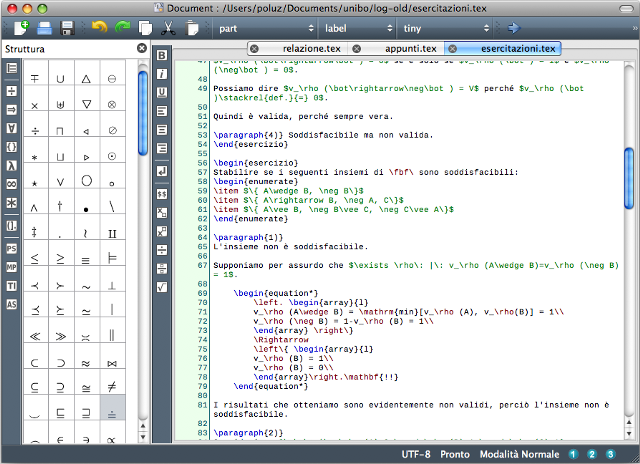
\includegraphics[scale=0.4]{images/texmaker.png}
\caption{Texmaker, A Graphical \LaTeX{} Editor}
\end{figure}
\item LEd
\begin{figure}[ht]
\centering
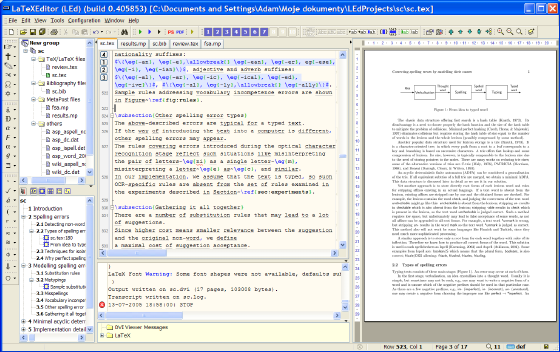
\includegraphics[scale=0.5]{images/led.png}
\caption{LEd, A Graphical \LaTeX{} Editor}
\end{figure}
\end{itemize}
And many more but the preferred method to produce \LaTeX{} document is through console mode only.


\subsection{Pdfscreen \LaTeX{}}
There are some packages that can help to have unified document using \LaTeX{}. Example of such a package is pdfscreen that let the user view it’s document in two forms-print and screen. Print for hard copy and screen for viewing your document on screen. Download this package from www.ctan.org/tex-archive/macros/latex/contrib/pdfscreen/.\\
Then install it using above mention method.\\

Just changing print to screen gives an entirely different view. But for working of pdfscreen another package required are comment and fancybox.\\

The fancybox package provides several different styles of boxes for framing and rotating content in your document. Fancybox provides commands that produce square-cornered boxes with single or double lines, boxes with shadows, and round-cornered boxes with normal or bold lines. You can box mathematics, floats, center, flushleft, and flushright, lists, and pages.\\

Whereas comments package selectively include/excludes portions of text. The comment package allows you to declare areas of a document to be included or excluded. One need to make these declarations in the preamble of your file. The package uses a method for exclusion that is pretty robust, and can cope with ill-formed bunches of text.\\

So these extra packages needed to be installed on system for the proper working of pdfscreen package.
\subsection{Web based graphic generation using \LaTeX{}}
\LaTeX{} is also useful when there is need of generating the graphics from browser. For
example to draw a circle by just entering its radius in html input box. So this kind
A
of project can be conveniently handled using \LaTeX{}. Basic idea behind this generation
process is that when user clicks on submit button after entering radius a script will run
that enter the radius in already made .tex file and recompiles it on server and makes its
pdf and postscript file. After that user can view those files by clicking on link provided
to view the files. See some screen shots of such a graphic generation project made by
Dr. H.S. Rai:\\

So here in the above input page which is also the index page user can enter input
for length of rectangle, breadth of rectangle and for radius of circle after that user can submit the values. After the values get submitted a script get runs by php code at server
side. This script first enters the dimensions of rectangle and circle that were selected by
user in to an already existing .tex file and replace with the older dimensions there. After
that script recompiles the the tex file and make it available for user.\\

In above figure it gets clear that .tex file has been compiled and pdf and postscript files
are available to user and user can download the graphics so produced. Hence graphics
can be generated in \LaTeX{} through web interface.
\begin{figure}[ht]
\centering
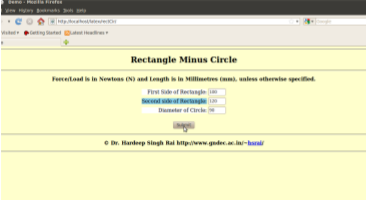
\includegraphics[scale=1]{images/webgraphic.png}
\caption{Web based graphic generation using \LaTeX{}(input page)}
\end{figure}

\section{Introduction to Doxygen}
\begin{figure}[h]
\centering 
\includegraphics[scale=1.3]{images/Doxygen.png}
\caption{Doxygen Logo}
\end{figure}
Doxygen is a documentation generator, a tool for writing software reference 
documentation. The documentation is written within code, and is thus 
relatively easy to keep up to date. Doxygen can cross reference 
documentation and code, so that the reader of a document can easily 
refer to the actual code.

Doxygen supports multiple programming languages, especially C++, C, 
C\#, Objective-C, Java, Python, IDL, VHDL, Fortran and PHP.[2] Doxygen
 is free software, released under the terms of the GNU General Public 
License.\\

\subsection{Features of Doxygen}
\begin{itemize}
\item Requires very little overhead from the writer of the documentation. 
Plain text will do, Markdown is support, and for more fancy or structured 
output HTML tags and/or some of doxygen's special commands can be used.
\item Cross platform: Works on Windows and many Unix flavors (including 
Linux and Mac OS X).
\item Comes with a GUI frontend (Doxywizard) to ease editing the options 
and run doxygen. The GUI is available on Windows, Linux, and Mac OS X.
\item Automatically generates class and collaboration diagrams in HTML 
(as clickable image maps) and $\mbox{\LaTeX}$ (as Encapsulated PostScript 
images).
\item Allows grouping of entities in modules and creating a hierarchy 
of modules.
\item Doxygen can generate a layout which you can use and edit to change 
the layout of each page.
\item Can cope with large projects easily.
\end{itemize}

\begin{figure}[H]
\centering 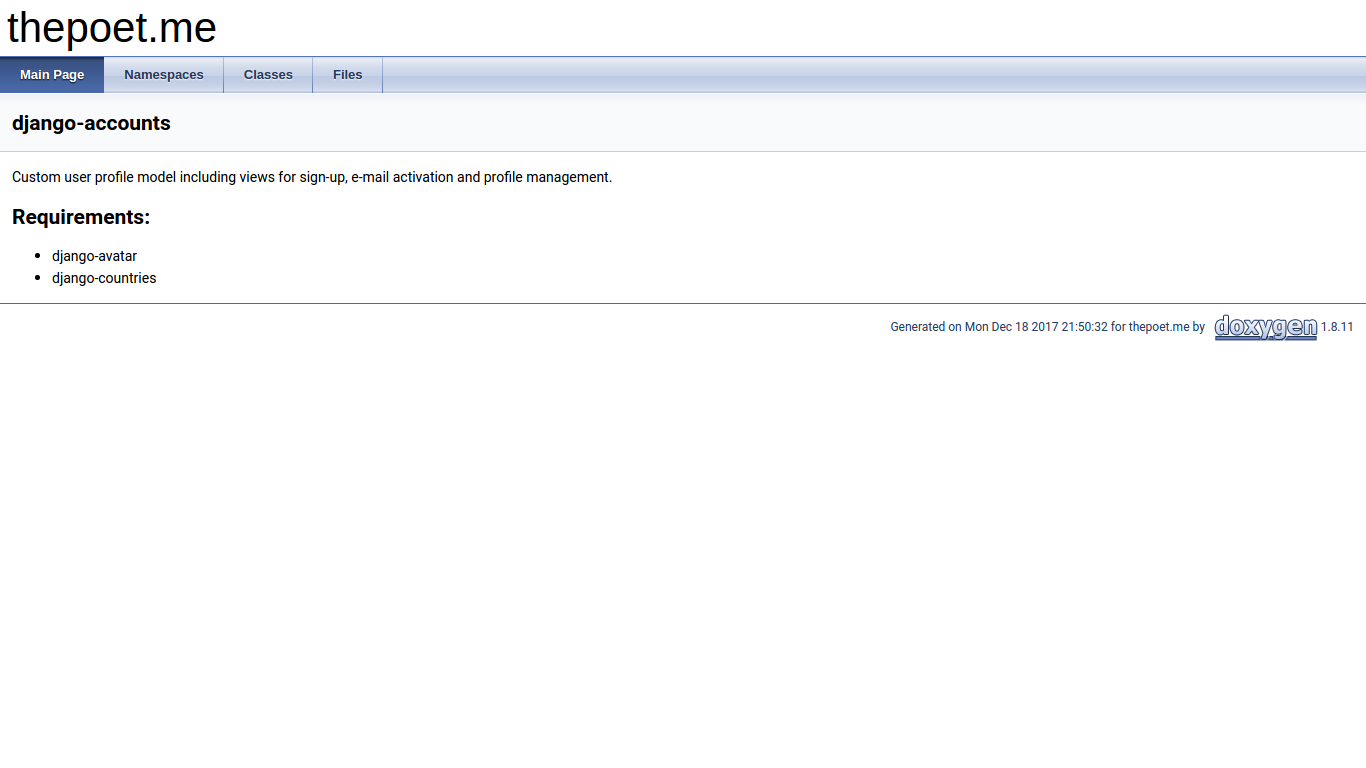
\includegraphics[scale=.35]{images/thepoetdoxy.png}
\caption{Documentation using Doxygen (main page)}
\end{figure}


\begin{figure}[H]
\centering 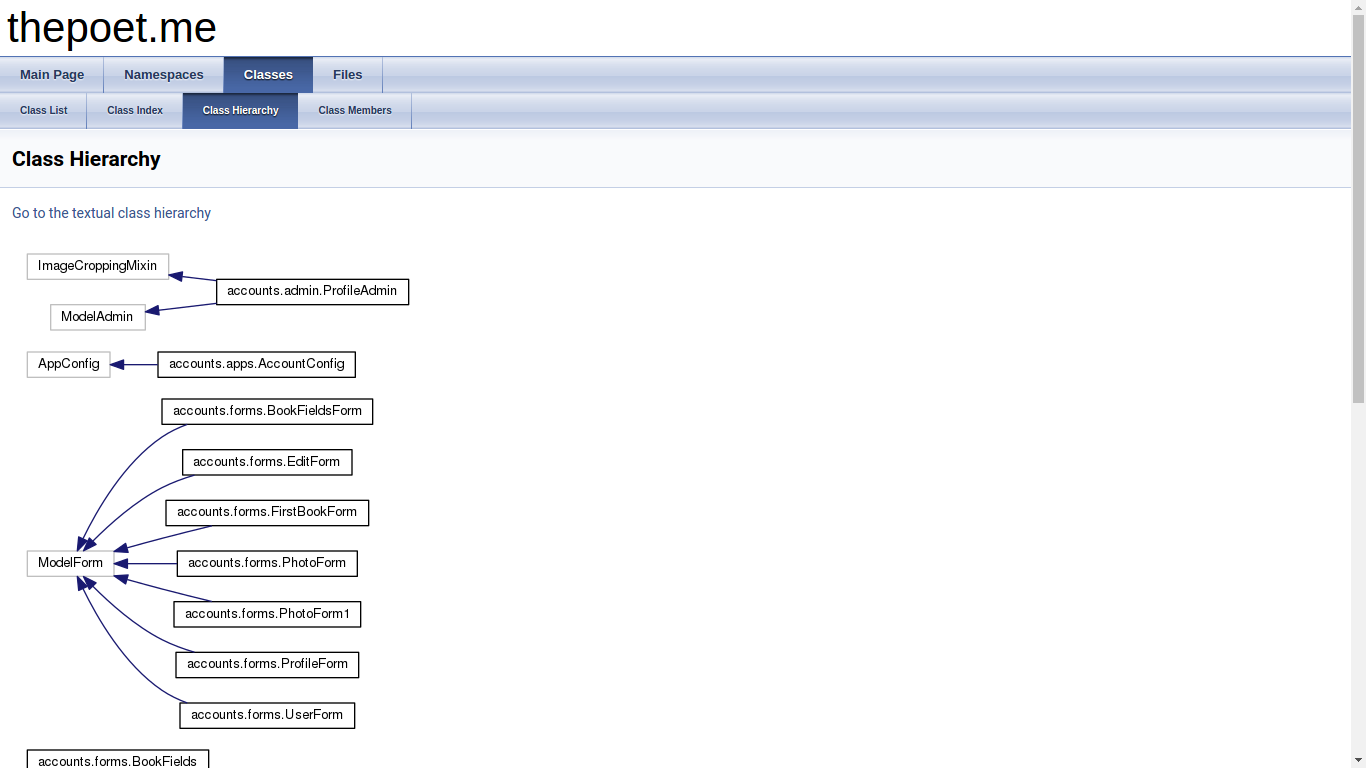
\includegraphics[scale=.35]{images/thepoetclass.png}
\caption{Doxygen documentation of a class hierarchy}
\end{figure}



\section{Introduction to Github}
\begin{figure}[!ht]
\centering

\includegraphics[width=0.3\textwidth]{images/github}                   
\caption{Github Logo}
\hspace{-1.5em}
\end{figure}
\leavevmode\\
GitHub is a Git repository web-based hosting service which offers all of the functionality of Git as well as adding many of its own features. Unlike Git which is strictly a command-line tool, Github provides a web-based graphical interface and desktop as well as mobile integration. It also provides access control and several collaboration features such as wikis, task management, and bug tracking and feature requests for every project.\\

GitHub offers both paid plans for private repto handle everything from small to very large projects with speed and efficiency. ositories, and free accounts, which are usually used to host open source software projects. As of 2014, Github reports having over 3.4 million users, making it the largest code host in the world.\\

GitHub has become such a staple amongst the open-source development community that many developers have begun considering it a replacement for a conventional resume and some employers require applications to provide a link to and have an active contributing GitHub account in order to qualify for a job.\\

The Git feature that really makes it stand apart from nearly every
other Source Code Management (SCM) out there is its branching model.\\
\\
Git allows and encourages you to have multiple local branches that can
be entirely independent of each other. The creation, merging, and
deletion of those lines of development takes seconds.\\ \\
This means that you can do things like:
\begin{itemize}
\item Frictionless Context Switching.\\ Create a branch to try out an
idea, commit a few times, switch back to where you branched from,
apply a patch, switch back to where you are experimenting, and merge
it in.
\item Role-Based Codelines. \\ Have a branch that always contains only
what goes to production, another that you merge work into for testing,
and several smaller ones for day to day work.
\item Feature Based Workflow. \\ Create new branches for each new
feature you're working on so you can seamlessly switch back and forth
between them, then delete each branch when that feature gets merged
into your main line.
\item Disposable Experimentation.\\  Create a branch to experiment in,
realize it's not going to work, and just delete it - abandoning the
work—with nobody else ever seeing it (even if you've pushed other
branches in the meantime).
\end{itemize}
Notably, when you push to a remote repository, you do not have to push
all of your branches. You can choose to share just one of your
branches, a few of them, or all of them. This tends to free people to
try new ideas without worrying about having to plan how and when they
are going to merge it in or share it with others.\\ \\
There are ways to accomplish some of this with other systems, but the
work involved is much more difficult and error-prone. Git makes this
process incredibly easy and it changes the way most developers work
when they learn it.

\subsection{What is Git?}
\begin{figure}[!ht]
\centering

\includegraphics[width=0.3\textwidth]{images/git}                   
\caption{Git Logo}
\hspace{-1.5em}
\end{figure}
Git is a distributed revision control and source code management (SCM) system with an emphasis on speed, data integrity, and support for distributed, non-linear workflows. Git was initially designed and developed by Linus Torvalds for Linux kernel development in 2005, and has since become the most widely adopted version control system for software development.\\

As with most other distributed revision control systems, and unlike most client–server systems, every Git working directory is a full-fledged repository with complete history and full version-tracking capabilities, independent of network access or a central server. Like the Linux kernel, Git is free and open source software distributed under the terms of the GNU General Public License version 2 to handle everything from small to very large projects with speed and efficiency.\\

Git is easy to learn and has a tiny footprint with lightning fast performance. It outclasses SCM tools like Subversion, CVS, Perforce, and ClearCase with features like cheap local branching, convenient staging areas, and multiple workflows.\\

\subsection{Installation of Git}

Installation of git is a very easy process.
The current git version is: 2.0.4.
Type the commands in the terminal:\\\\
\emph{
\$ sudo apt-get update\\\\
\$ sudo apt-get install git\\\\}
This will install the git on your pc or laptop.

\subsection{Various Git Commands}

Git is the open source distributed version control system that facilitates GitHub activities on your laptop or desktop. The commonly used Git command line instructions are:-\\

\subsubsection{Create Repositories}
Start a new repository or obtain from an exiting URL

\begin{description}

\item [\$ git init [ project-name]]\\
Creates a new local repository with the specified name
\item [\$ git clone [url]]\\
Downloads a project and its entire version history\\

\end{description}


\subsubsection{Make Changes}
Review edits and craft a commit transaction

\begin{description}

\item [\$ git status] \leavevmode \\
Lists all new or modified files to be committed

\item [\$ git diff] \leavevmode \\
Shows file differences not yet staged

\item [\$ git add [file]]\\
Snapshots the file in preparation for versioning

\item [\$ git reset [file]]\\
Unstages the file, but preserve its contents

\item [\$ git commit -m "[descriptive message]"]\\
Records file snapshots permanently in version history\\

\end{description}


\subsubsection{Group Changes}
Name a series of commits and combine completed efforts

\begin{description}

\item [\$ git branch] \leavevmode \\
Lists all local branches in the current repository

\item [\$ git branch [branch-name]]\\
Creates a new branch

\item [\$ git checkout [branch-name]]\\
Switches to the specified branch and updates the working directory

\item [\$ git merge [branch]]\\
Combines the specified branch’s history into the current branch

\item [\$ git branch -d [branch-name]]\\
Deletes the specified branch\\

\end{description}


\subsubsection{Save Fragments}
Shelve and restore incomplete changes

\begin{description}

\item [\$ git stash] \leavevmode \\
Temporarily stores all modified tracked files

\item [\$ git stash pop] \leavevmode \\
Restores the most recently stashed files

\item [\$ git stash list] \leavevmode \\
Lists all stashed changesets

\item [\$ git stash drop] \leavevmode \\
Discards the most recently stashed changeset\\

\end{description}


\subsubsection{Synchronize Changes}
Register a repository bookmark and exchange version history

\begin{description}

\item [\$ git fetch [bookmark]]\\
Downloads all history from the repository bookmark

\item [\$ git merge [bookmark]/[branch]]\\
Combines bookmark’s branch into current local branch

\item [\$ git push [alias][branch]]\\
Uploads all local branch commits to GitHub

\item [\$ git pull] \leavevmode \\
Downloads bookmark history and incorporates changes

\end{description}


\section{Implementation}
\subsection{Customizer}

\begin{figure}
	\centering 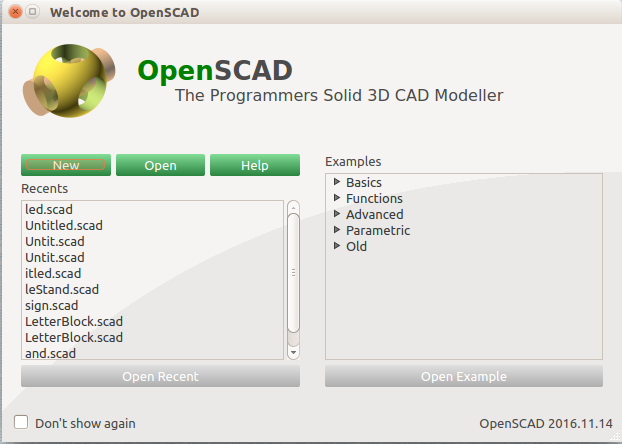
\includegraphics[scale=0.60]{images/output/1.png}
	\caption{StartUp Screen for OpenSCAD}
	\label{fig:1}
\end{figure}

Customizer  will provide User Interface to Customize Models interactively instead of modifying them manually. It will make the user able to create the templates for given model which can further be customized to cater to their need of different users and also provide a feature to save the set of parameters which define a different model using the same template of the model.
\subsection{Activation of Customizer functions}
\begin{itemize}
	
	\item This is experimental functionality.So, Initially
	OpenSCAD will look like \ref{fig:Normal OpenSCAD}
	\item In [Edit] menu, select [Preferencews] then open tab [Features], tick Customizer, then close the window when tick shown \ref{fig:3}.
	\item In View menu, you shall now have an option [Hide customizer], that you shall untick. Then you will be able to see the customizer \ref{fig:OpenSCAD with Customizer}
	
\end{itemize}

\begin{figure}
	\centering 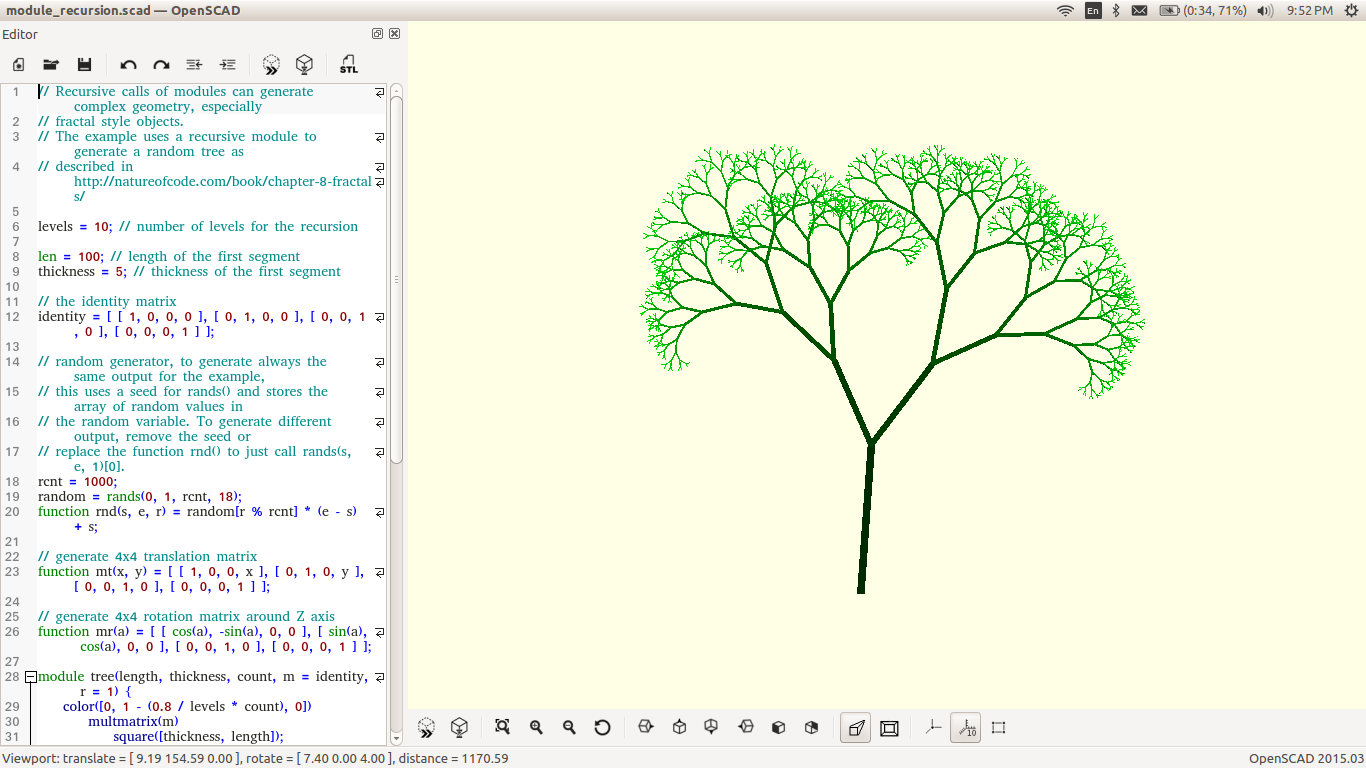
\includegraphics[width=\linewidth]{images/output/2.png}
	\caption{OpenSCAD without customizer}
	\label{fig:Normal OpenSCAD}
\end{figure}
\begin{figure}
	\centering 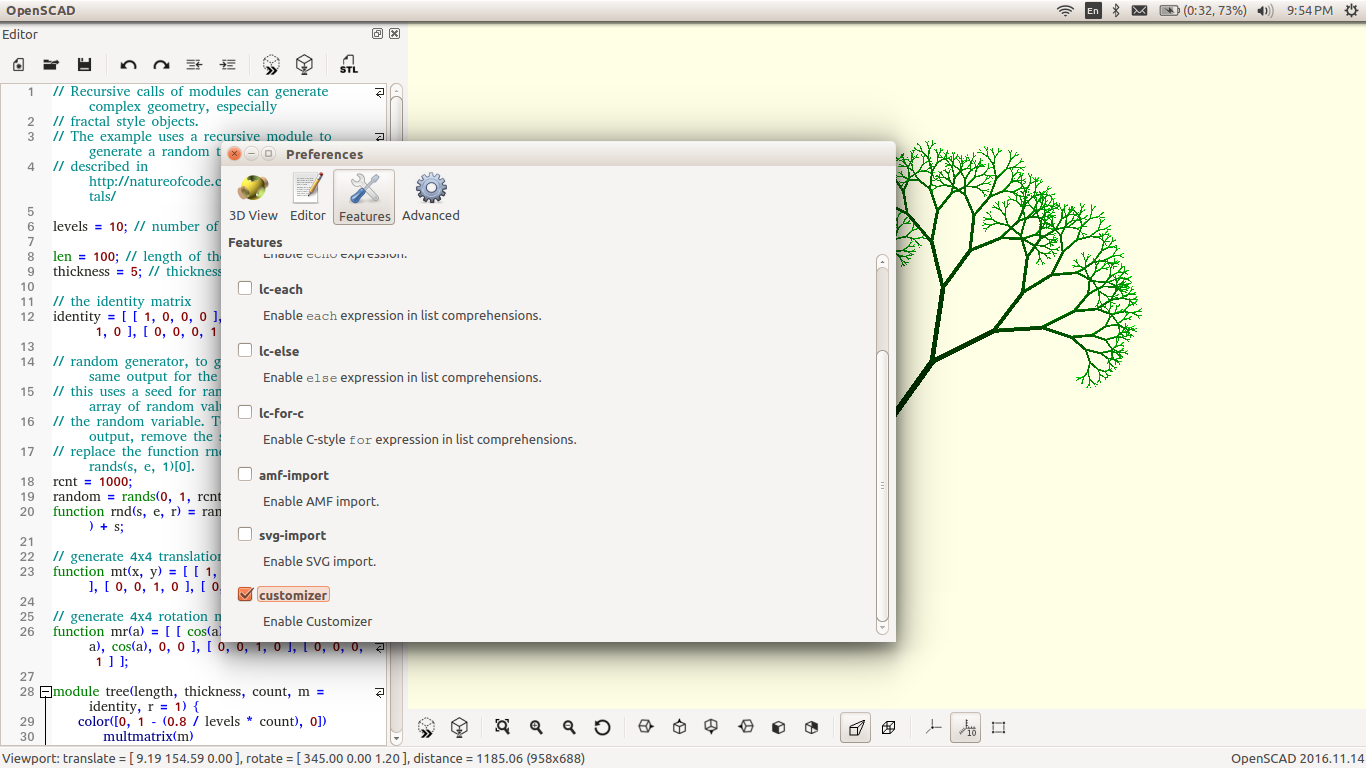
\includegraphics[width=\linewidth]{images/output/3.png}
	\caption{Preferences Widget to activate Customizer}
	\label{fig:3}
\end{figure}
\begin{figure}
	\centering 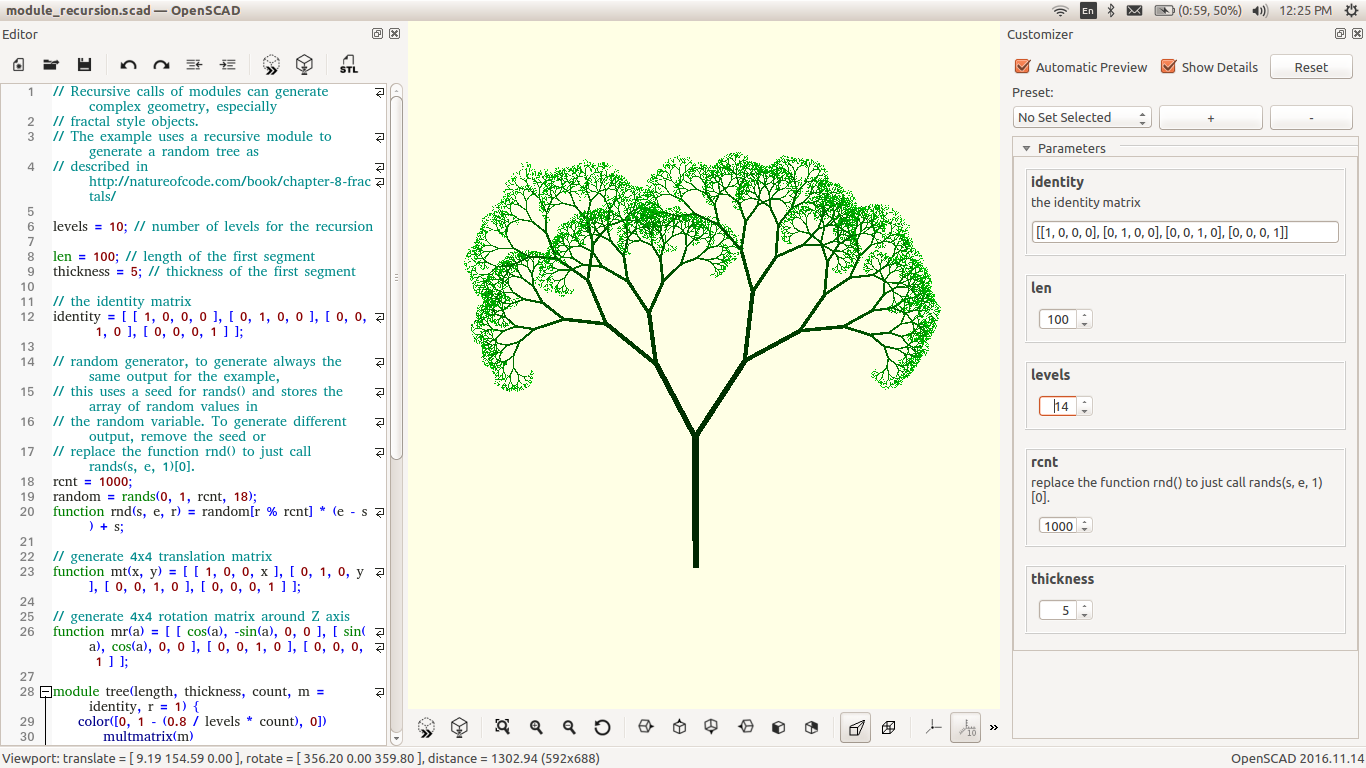
\includegraphics[width=\linewidth]{images/output/5.png}
	\caption{OpenSCAD with Customizer }
	\label{fig:OpenSCAD with Customizer}
\end{figure}

\subsection{Syntax support for generation of the customization form}

\begin{lstlisting}[language=c++]
// variable description
variable name = defaultValue; // possible values
\end{lstlisting}

Parameter will be decorated with meta data using the comments and the single line comments above the parameter could be used to describe the meaning of the parameter and its use. The comments in same line as that of parameter is used to define the GUI that have to be used to modify that values of that parameter.

Following is the syntax for how to define different types of widgets in the form

\begin{enumerate}
	\item \textbf{Drop down box:} \ref{fig:example} Following type of comboBox could be created with following syntax:
	\begin{figure}
		\centering
		\includegraphics[width=\linewidth]{images/example}
		\caption{Shows the different types ComboBox, Slider}
		\label{fig:example}
	\end{figure}
	
	\begin{lstlisting}[language=c++]
	// combo box for nunber
	Numbers=2; // [0, 1, 2, 3]
	
	// combo box for string
	Strings="foo"; // [foo, bar, baz]
	
	//labeled combo box for numbers
	Labeled_values=10; // [10:L, 20:M, 30:L]
	
	//labeled combo box for string
	Labeled_value="S"; // [S:Small, M:Medium, L:Large]
	\end{lstlisting}
	\item \textbf{Slider:} Only numbers are allowed in this one, \ref{fig:example} specify any of the following:
	\begin{lstlisting}[language=c++]
	// slider widget for number
	slider =34; // [10:100]
	
	//step slider for number
	stepSlider=2; //[0:5:100]
	\end{lstlisting}
	\item \textbf{Checkbox:} \ref{fig:example1} Following widget is created with given syntax:
	\begin{lstlisting}[language=c++]
	//description
	Variable = true;
	\end{lstlisting}
	\item \textbf{Spinbox:} \ref{fig:example1} Following widget is created with given syntax:
	\begin{lstlisting}[language=c++]
	// spinbox with step size 1
	Spinbox= 5;
	
	// spinbox with step size 0.01
	Spinbox= 5.11;
	
	//spinbox with given step size
	SpinboxWithStep= 5; //2
	\end{lstlisting}
	\item \textbf{Textbox:} \ref{fig:example1} Following widget is created with given syntax:
	\begin{lstlisting}[language=c++]
	//Text box for vector with more than 4 elements
	Vector=[12,34,44,43,23,23];
	
	// Text box for string
	String="hello";
	
	\end{lstlisting}
	\item \textbf{Special vector:} \ref{fig:example1} Following widget is created with given syntax:
	\begin{lstlisting}[language=c++]
	
	//Text box for vector with less than or equal to 4 elements
	Vector2=[12,34,45,23];
	\end{lstlisting}
	\begin{figure}
		\centering
		\includegraphics[width=\linewidth]{images/example1}
		\caption{Shows the CheckBox, TextBox, SpinBox, VectorWidget}
		\label{fig:example1}
	\end{figure}
	
\end{enumerate}

\subsection{Creating Tabs}
Parameters can be grouped into \textbf{tabs}. This feature will allow us to separate similar and related parameters. The syntax for this is also mainly similar to that of Thingiverse syntax for creating the tabs. To create a tab, use a multi-line block comment like this:

\textbf{/* [Tab Name] */}


Screenshot number \ref{fig:5} Shows the implemenation of this feature.

The following tab names are reserved for special functionality:
\begin{description}
	\item [Global] Parameters in the global tab will always be shown on every tab no matter which tab is selected. Note: there will be no tab for “Global” params, they will just always be shown in all the tabs.
	
	\item [Hidden] Parameters in the hidden tab will never be displayed. Not even the tab will be shown. Even though the variables who have not been parameterized using the Thingiverse or native syntax will not be displayed in OpenSCAD parameter widget but we have implemented this to make our comment like syntax similar as that of Thingiverse.
\end{description}

Also, the parameters who are under no tab will be displayed under TAB named “parameters”.
\begin{lstlisting}[language=c++]
// combo box for nunber
Numbers=2; // [0, 1, 2, 3]

// combo box for string
Strings="foo"; // [foo, bar, baz]


/*[ Slider ]*/
// slider widget for number
slider =34; // [10:100]

//step slider for number
stepSlider=2; //[0:5:100]

/* [Global] */

//description
Variable = true;

/*[Hidden] */

// spinbox with step size 1
Spinbox = 5;

/* [Textbox] */

//Text box for vector with more than 4 elements
Vector=[12,34,44,43,23,23];

// Text box for string
String="hello";

\end{lstlisting}

\begin{figure}
	\centering 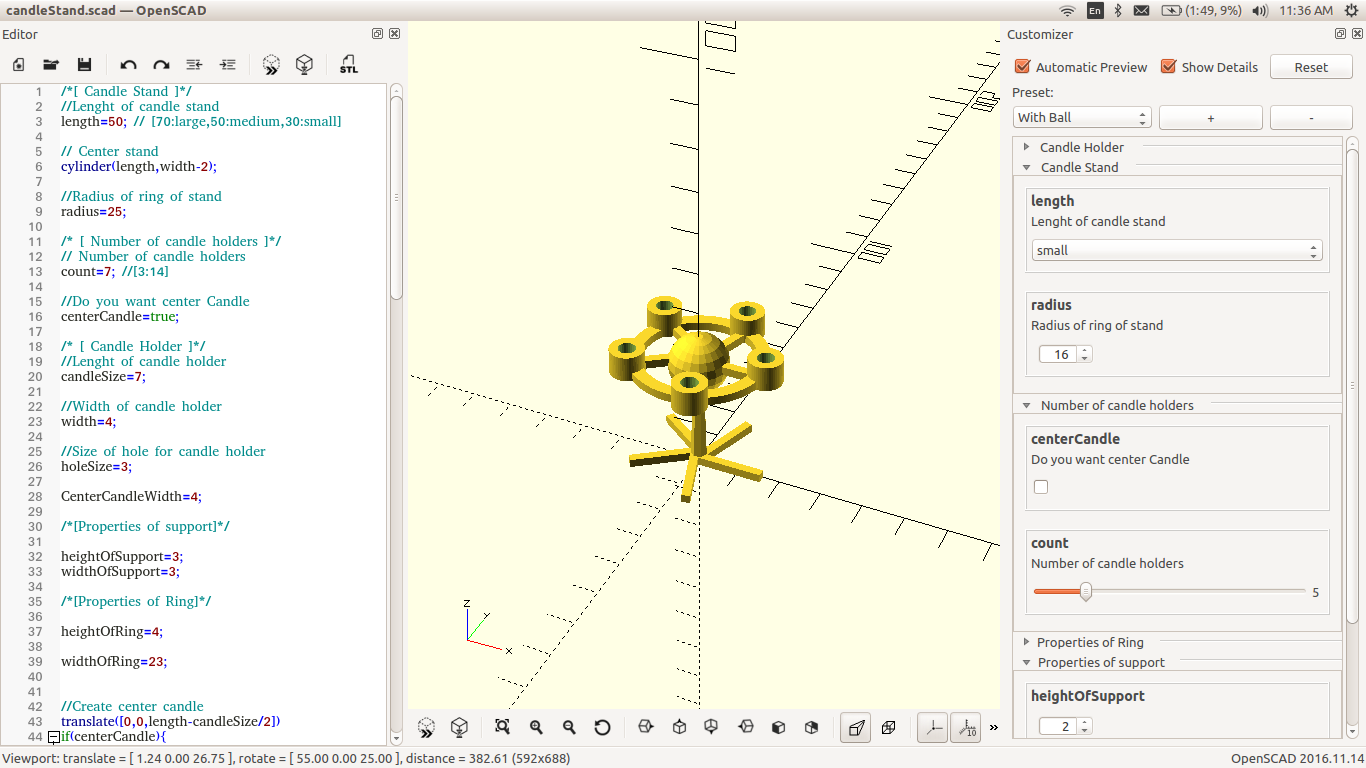
\includegraphics[width=\linewidth]{images/output/6.png}
	\caption{Shows different groups generated through customzier}
	\label{fig:5}
\end{figure}

\addcontentsline{toc}{chapter}{BIBLIOGRAPHY}
\bibliographystyle{ieeetr} 
\begin{thebibliography}{22}



\bibitem{} "Jagjeet Singh", Blog, 2017. [Online]. Available: https://jagjeet.me. [Accessed: 27- Nov- 2017].

\bibitem{} "Doxygen: Main Page", Doxygen.org, 2017. [Online]. Available: http://www.doxygen.org. [Accessed: 27- Nov- 2016].

\bibitem{} "Django" docs, 2017. [Online]. Available: https://www.djangoproject.com. [Accessed: 27- Nov- 2016].

\bibitem{} "Git", En.wikipedia.org, 2017. [Online]. Available: 
https://en.wikipedia.org/wiki/Git. [Accessed: 27- Nov- 2017].

\bibitem{} "Python", En.wikipedia.org, 2017. [Online]. Available: https://en.wikipedia.org/wiki/Python. [Accessed: 27- Nov- 2017].

\end{thebibliography}



\end{document}

